\chapter[Secure Public Verification of Generative-AI Provenance]{Secure Public Verification of Generative-AI Provenance: PP-Mark}
\label{ch:pp-mark}

\section{Introduction}
\label{sec:ch4-introduction}

The preceding two chapters developed the \AuditablePrivacy{} axis of this
dissertation.  They asked whether a privacy sentence is licensed by a completed
execution and whether a requested privacy route is coherently assembled before
that execution begins.  This chapter turns to a separate trust claim: whether a
third party can verify that a generated image is accompanied by evidence
consistent with a declared generation context.  The protected object, mechanism,
and evidence are different, but the assurance problem has the same form.  A
positive label should not be released merely because one observable statistic
crosses a threshold; the label must remain aligned with the process and evidence
that give it meaning.

Image provenance has become harder to establish as generative models have
improved.  Synthetic images can support benign creation, accessibility, and
simulation, but they can also be used for impersonation and misleading media.
The resulting provenance problem is not solved by visual inspection
alone~\cite{chesney2019deepfakes,longpre2024provenance}.  Content credentials and
signed metadata provide an important publication layer, yet the strength of a
provenance claim still depends on what the attached technical evidence actually
establishes~\cite{c2pa2026spec}.  A signature can authenticate a manifest supplied
by a key holder.  It does not, by itself, show that a registered watermark signal
was embedded according to the process named in that manifest.

Digital watermarking addresses this gap by placing a recoverable signal in the
image or in the generative process.  Post-hoc methods encode a message after an
image is produced, while latent and model-integrated methods introduce structured
signals during generation~\cite{zhu2018hidden,tancik2020stegastamp,
wen2023treerings,fernandez2023stablesignature}.  Verification commonly evaluates a
detector $D(I,\mathrm{md})$ and accepts when its score exceeds a calibrated
threshold.  This design offers low latency and can remain useful after moderate
compression or transformation.  Its weakness is also structural: once the
detector is public, the same decision surface that enables independent checking
becomes a target for queries, surrogate construction, or gradient-based
optimization~\cite{jiang2023evading,muller2025blackbox,lin2025crack}.

Keeping the detector private behind an application programming interface reduces
direct exposure but replaces technical verification with organizational trust.
Only the service operator can execute the hidden rule, rate-limit queries, or
resolve disputes.  A user cannot reproduce the judgment independently, and a
long-lived provenance record remains dependent on the continued availability and
integrity of one verifier.  Public verification and forgery resistance therefore
appear to pull in opposite directions: opening the detector improves auditability
but expands the attack surface, whereas closing it reduces independent
auditability.

This chapter studies \PPMark{}, a construction that changes the acceptance rule
rather than merely hiding or hardening the score.  The generator derives a latent
watermark from a secret-keyed binding to the prompt, seed, model identifier, and
resolution.  It commits a deterministic sample of the embedding trace under a
Merkle root and produces an SP1 zero-knowledge proof receipt.  A public verifier
recovers a statistical watermark score from the submitted image and verifies the
receipt against the declared context, the committed trace, and the exact
canonical image hash.  Full acceptance requires both conditions:

\begin{equation}
\begin{aligned}
    &\mathsf{PPMark}_{\mathrm{accept}}(I,\mathrm{md},\PPReceipt)=1\\
    &\quad\Longleftrightarrow
    \bigl(\PPDetectionScore(I,\mathrm{md})\geq\PPThreshold\bigr)
    \land
    \bigl(\mathsf{VerifyReceipt}(\PPReceipt;\PPPublicStatement)=1\bigr).
\end{aligned}
\label{eq:ch4-intro-accept}
\end{equation}

Equation~\eqref{eq:ch4-intro-accept} is the chapter's central claim-alignment
boundary.  The score provides image-side evidence that the expected signal is
recoverable.  The receipt provides process-side evidence that the opened committed
trace is consistent with a secret-key-derived binding and an image-bound challenge.
Neither term is promoted into the other.  A high score alone is a screening
result, not publicly verified provenance, and a valid receipt alone does not show
that the published pixels retain the detectable signal.

The contributions of this chapter are summarized as follows.

\begin{itemize}
    \item It formulates secure public provenance verification as a conjunctive
    evidence decision.  The public detector remains available for low-latency
    screening, while a stronger acceptance mode additionally requires a
    cryptographic receipt bound to the declared generation context and exact
    image.

    \item It defines a context-bound latent watermark.  A secret-keyed binding
    determines a Reed--Solomon payload, sampled latent positions, Gaussian
    baselines, and signed perturbations.  The same binding therefore anchors the
    statistical sign pattern and the proof predicate.

    \item It commits sampled trace tuples and verifies a randomized opening in an
    SP1 zkVM.  The construction states the public/private split explicitly and
    gives a conditional unforgeability bound containing hash, proof-system, and
    partial-opening failure terms.

    \item It evaluates the two verification modes against fabricated bindings,
    compliance bypass, black-box imprint transfer, white-box optimization,
    regeneration, steganalysis, and common image transformations.  It also records
    the proving, verification, receipt-size, quality, and two-model limits
    needed to interpret the result operationally.
\end{itemize}

The assurance boundary is deliberately narrower than proof of image truth or
authorship.  \PPMark{} does not determine whether the prompt is factually correct,
whether the depicted event occurred, whether a person owns a legal identity, or
whether every diffusion operation was faithfully executed.  Its circuit does not
re-simulate the full diffusion model.  It verifies the declared composite relation
over a committed sampled trace, and full acceptance is meaningful only under the
stated hash, proof-system, key-secrecy, predicate, statistical, and partial-opening
assumptions.  The correct conclusion is therefore that an accepted image carries
verifiable provenance evidence relative to the declared binding, not that the
image is unconditionally authentic.

\section{Background and Related Work}
\label{sec:ch4-background}

\subsection{Generative Image Watermarking and Provenance}
\label{subsec:ch4-watermark-background}

An image-watermarking system normally exposes three logical procedures.  An
embedding procedure receives an image or generation state and a payload; an
extraction procedure recovers a message or statistic from a candidate image; and a
decision procedure compares the recovered object with a reference or threshold.
These procedures can be placed at different points in the image pipeline.

Post-hoc watermarking changes the completed pixel image.  HiDDeN learns an
encoder--decoder pair for hiding data in images, StegaStamp targets robustness
under physical and geometric transformations, and more recent systems such as
TrustMark and InvisMark improve capacity or robustness at arbitrary image
resolutions~\cite{zhu2018hidden,tancik2020stegastamp,bui2025trustmark,
xu2025invismark}.  Post-hoc deployment is attractive because it can wrap an
existing generator.  At the same time, the watermark is separated from the
internal generation path and may be attenuated by regeneration or model-based
removal~\cite{zhao2024removable}.

Generative or semantic watermarking moves the signal into the model or latent
trajectory.  Tree-Ring introduces structured patterns in initial diffusion noise,
Gaussian Shading encodes a lossless latent distribution, and Stable Signature
roots a watermark in a latent-diffusion decoder~\cite{wen2023treerings,
yang2024gaussianshading,fernandez2023stablesignature}.  RingID extends ring-based
signals to multi-key identification, while WIND separates watermark detection into
two stages for public use~\cite{ci2024ringid,arabi2025wind}.  These methods differ
in payload, perceptual objective, and robustness profile, but their common public
interface is still usually a detector score or decoded identity.

Provenance requires a more precise interpretation than watermark presence.  A
positive score means that the submitted image resembles the detector's expected
signal strongly enough under a calibration rule.  It does not necessarily bind
that signal to one prompt, seed, model, resolution, or committed execution trace.
Likewise, signed content credentials authenticate the signed assertions and their
chain, but the assertion is only as strong as the evidence placed behind it.  The
technical question in this chapter is consequently not whether statistical
watermarks or signed manifests should be discarded.  It is how a public
watermark decision can be coupled to a separately checkable relation describing
the claimed generation context.

This distinction yields two complementary service levels.  A statistical mode can
scan large volumes of transformed images and tolerate small signal degradation.  A
proof-bearing mode can make a stronger statement about an exact published object,
but must carry an explicit proof artifact and generally rejects altered pixels.
Treating these modes as interchangeable would obscure both their value and their
limits.

\subsection{Forgery Vulnerabilities of Public Detectors}
\label{subsec:ch4-public-detector-forgery}

A removal attack begins with a watermarked image and tries to lower its detection
score while preserving acceptable image quality.  A forgery attack begins with an
unmarked or differently marked image and tries to raise the score associated with
a target source.  These goals are asymmetric.  Robustness against removal does not
imply resistance to forgery, because a highly stable but publicly exposed pattern
may be easy to implant in unrelated content.

Black-box imprint attacks demonstrate this distinction.  From a watermarked
reference, the adversary estimates a transferable imprint and optimizes an
arbitrary cover image so that a target detector attributes it to the reference
source~\cite{muller2025blackbox}.  The attack does not require disclosure of the
target scheme's internal key derivation.  Query access, proxy models, and common
latent structure can supply a useful optimization signal.  A successful attack
therefore produces a positive detector outcome without the generation process
that the verifier may implicitly associate with that outcome.

The white-box case is stronger.  When the detector or a differentiable surrogate
is public, an adversary can maximize the verification statistic directly under a
pixel perturbation budget.  Prior work shows that watermark-based detectors can be
evaded or optimized against when their decision rules are exposed, and public
knowledge of a watermark's structure can enable specialized removal
strategies~\cite{jiang2023evading,lin2025crack}.  Rate limits may slow a pure
query attack, but they do not create cryptographic evidence that a positive score
originated from the registered embedder.

A signature-only construction addresses a different object.  If metadata is
signed, an adversary without the signing key cannot alter it undetectably.  If the
signing key is available to a malicious producer or compromised operator,
however, the attacker can sign a fabricated binding or a clean image.  Adding a
score blocks the clean-image case only when the attacker cannot search for a
binding whose derived pattern happens to correlate with the image.  The resulting
problem is a claim--evidence mismatch: the public interface says ``verified,'' but
the evidence may show only that some chosen detector statistic crossed a threshold
and some metadata was signed.

The threat model used here grants the adversary watermarked images and all public
artifacts.  The adversary may manipulate pixels, query the public score, and use
detector gradients.  The PP-Mark binding key \PPSecretKey{} is not disclosed, and
the adversary is assumed unable to violate SHA-256 collision resistance or SP1
computational soundness.  A conventional metadata-signing key used in comparison
architectures is separate from \PPSecretKey{}; compromising that comparison key
does not reveal the PP-Mark binding key.  Conversely, compromise of
\PPSecretKey{} is an explicit failure of the operational assumption and is not
hidden by the theorem.

\subsection{Zero-Knowledge Proofs and Verifiable Computation}
\label{subsec:ch4-zkp-background}

Commit-and-open protocols allow a prover to fix a large object before learning
which parts a verifier will inspect.  A Merkle tree reduces the committed object
to one root; an authentication path then proves that an opened leaf belongs to the
committed tree without publishing every leaf~\cite{merkle1988signature}.  If the
opening challenge is derived after the commitment and is bound to the submitted
image, a prover cannot freely reuse one favorable opening for a different image.
The residual risk is explicit: a random opening can miss all positions at which a
committed trace cheats.  That probability becomes a term in the guarantee rather
than an implicit trust assumption.

Zero-knowledge proofs add a second property.  A prover can demonstrate that a
private witness satisfies a public predicate without revealing the witness itself.
PP-Mark realizes this layer with the SP1 zero-knowledge virtual machine, which can
prove execution of a Rust program and publish a standalone receipt~\cite{roy2024sp1}.
The proof program checks key binding, Merkle commitment, image-bound challenge,
and deterministic embedding relations.  It does not prove the semantic truth of
the context fields, and it does not re-run the complete image generator.

Related provenance systems occupy adjacent points in this design space.  C2PA
standardizes signed content credentials and manifest relationships, whereas
PP-Mark supplies evidence about a watermark embedding relation that can be carried
with such metadata~\cite{c2pa2026spec}.  VeriLLM uses commitment and randomized
opening to make decentralized inference publicly checkable; PP-Mark applies a
related commit--open--verify idea to sampled image-watermark traces and additionally
binds the opening challenge to the exact image hash~\cite{wang2025verillm}.
ZeroMark hides a dataset watermark during ownership verification, and CLUE-Mark
studies undetectability from a lattice assumption; those goals are complementary
to the unforgeability target studied here~\cite{guo2024zeromark,
shehata2024cluemark}.

The key design decision is thus not the mere presence of a zero-knowledge proof.
The public statement must name the same binding and image used by the score, the
private witness must encode the committed trace relation, and the final interface
must refuse to collapse a score-positive result into full acceptance.  Otherwise,
a proof can be valid while remaining irrelevant to the provenance sentence shown
to the user.

\section{PP-Mark}
\label{sec:ch4-method}

Figure~\ref{fig:ch4-overview} presents the complete data flow.  During generation,
the context and secret key derive a public binding; that binding drives both the
latent sign pattern and the trace commitment.  The generator publishes metadata,
a Merkle root, and a proof receipt alongside the image.  During verification, a
third party inverts the image to estimate its initial latent, recomputes the score,
hashes the canonical pixels, and verifies the receipt.  No central detector API or
disclosure of the binding key is required.

\begin{figure}[H]
    \centering
    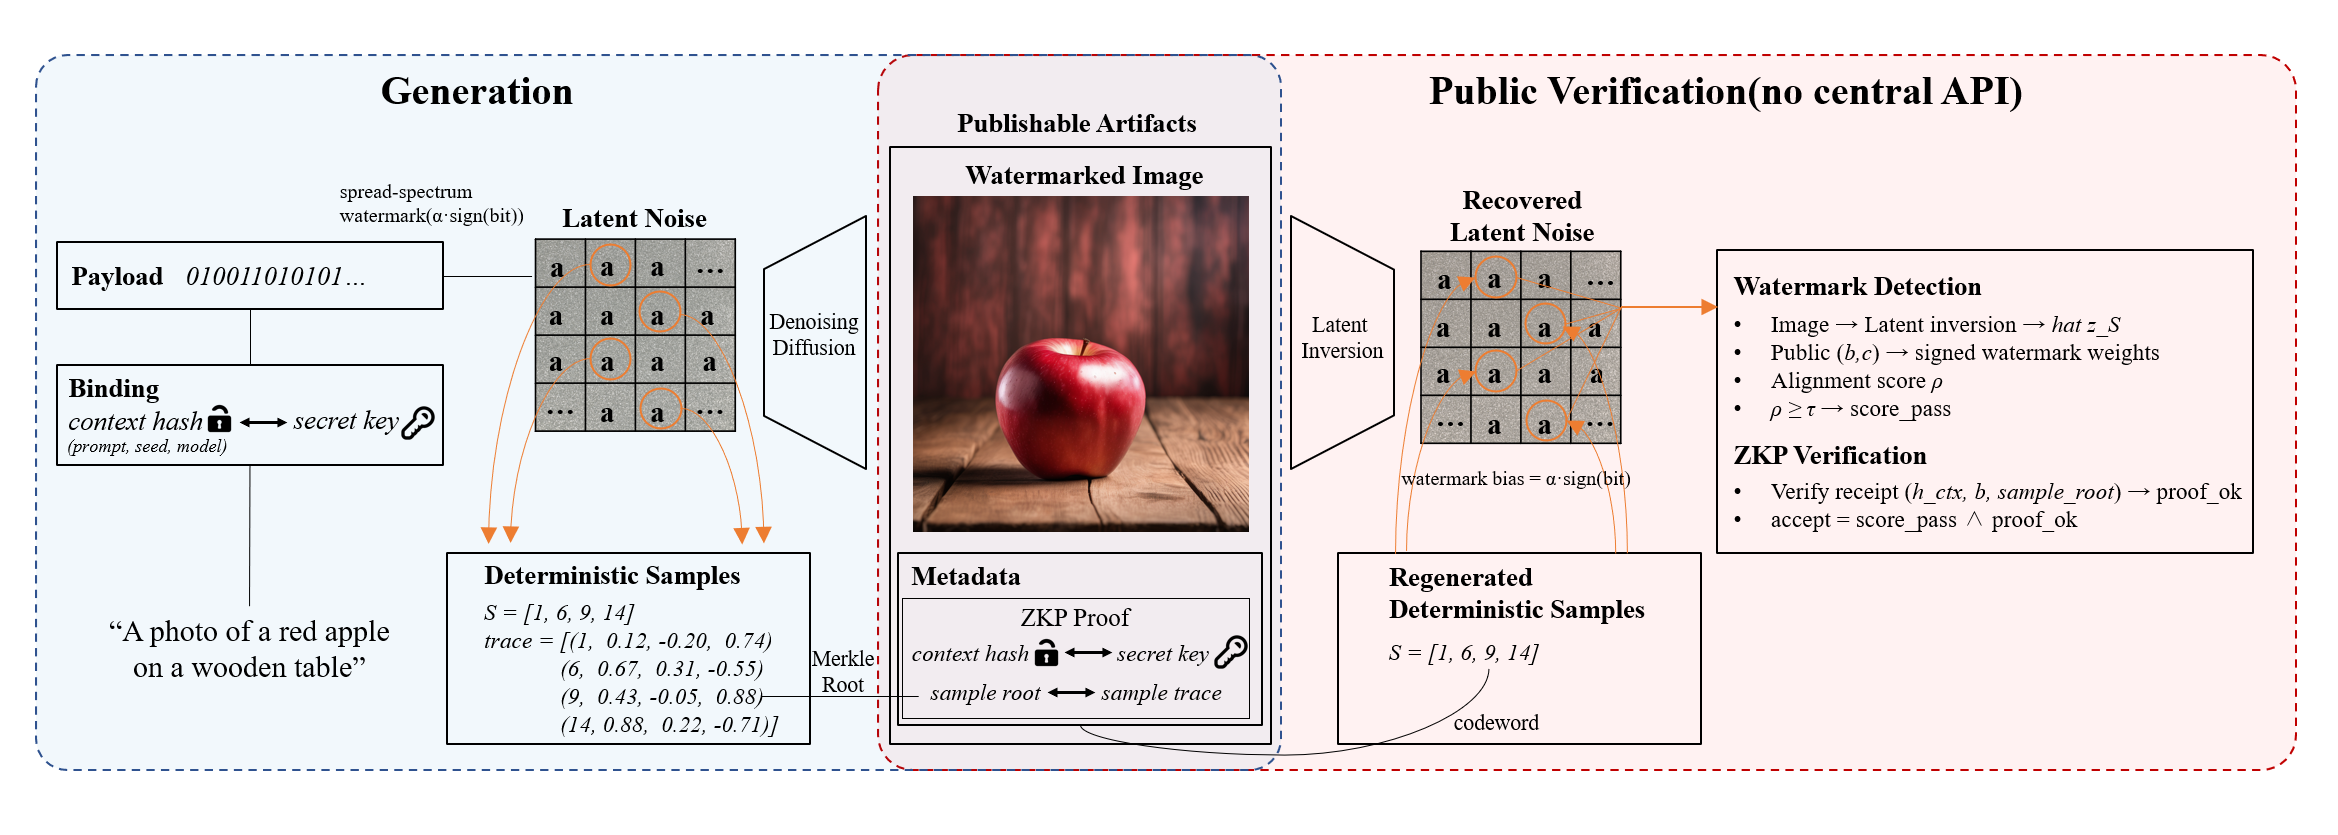
\includegraphics[width=\textwidth]{figures/ch04_source_ppmark_overview.png}
    \caption{PP-Mark generation and public verification workflow}
    \label{fig:ch4-overview}
\end{figure}

\subsection{Context-Bound Binding and Payload Construction}
\label{subsec:ch4-binding-payload}

Let $p$ be the prompt, $s$ the generation seed, \PPModelID{} the model
identifier, and $W\times H$ the output resolution.  Domain-separated hashing
first constructs a context hash and then mixes that public context with the secret
binding key:

\begin{equation}
\begin{aligned}
    h_p
        &= H(p),\\
    \PPContextHash
        &= H(\texttt{ctx\_hash}\parallel h_p\parallel\PPModelID\parallel
             s\parallel W\parallel H),\\
    \PPBinding
        &= H(\texttt{ctx\_hash}\parallel\PPContextHash\parallel\PPSecretKey).
\end{aligned}
\label{eq:ch4-binding-chain}
\end{equation}

Changing the prompt, seed, model identifier, or resolution changes
\PPContextHash{} and hence \PPBinding{}.  The prompt itself need not be placed in
the proof witness; its digest is sufficient for the binding relation.  Domain
separation prevents the same hash invocation from being interpreted as another
protocol field.

The public binding becomes a fixed-length watermark message and codeword:

\begin{equation}
    \PPPayload=\operatorname{Trunc}(\PPBinding),
    \qquad
    \PPCodeword=\operatorname{RS}(\PPPayload),
    \qquad
    \mathbf{r}=\operatorname{Bits}(\PPCodeword).
\label{eq:ch4-payload-codeword}
\end{equation}

Reed--Solomon expansion supplies a redundant binary sequence \(\mathbf r\) that
can be spread across the latent space.  This sequence is public once \PPBinding{}
is published, but the proof must still show that \PPBinding{} is consistent with a
valid secret-key witness.  Public reconstructability is necessary for independent
score computation; it is not permission to choose a new binding after inspecting
the target image.

The exact image enters after the trace has been committed.  Let
\(\mathsf{root}_{\mathrm{tr}}\) denote the Merkle root of the sampled trace and let
\PPImageHash{} be SHA-256 of deterministically canonicalized pixels.  The public
challenge material is

\begin{equation}
\begin{aligned}
    u
        &= (\PPImageHash,\PPContextHash,\mathsf{root}_{\mathrm{tr}}),\\
    \mathsf{seed}_{\mathrm{open}}
        &= H(\texttt{ppmark\_opening\_v1}\parallel u),\\
    \PPOpeningSet
        &= \operatorname{DeriveOpen}
           (\mathsf{seed}_{\mathrm{open}},\PPOpeningCount,\PPSampleCount).
\end{aligned}
\label{eq:ch4-opening-challenge}
\end{equation}

This ordering matters.  The root fixes the trace before the opening set is known,
and \PPImageHash{} prevents a receipt prepared for one exact image from being
replayed unchanged on another.  A cryptographic pixel hash is chosen instead of a
perceptual hash because a perceptual collision neighborhood would create an
explicit replay region.  The consequence is intentional but operationally
important: recompression, crop, resize, or any other pixel change invalidates the
receipt and requires proof re-issuance for the edited variant.

\subsection{Deterministic Sampling and Latent Watermark Embedding}
\label{subsec:ch4-sampling-embedding}

The codeword deterministically selects \PPSampleCount{} latent locations,

\begin{equation}
    \PPSampleSet
        =\operatorname{DeterministicSample}
          (\PPCodeword,\PPSampleCount),
    \qquad
    \operatorname{idx}(x,y)
        =H(\PPBinding\parallel x\parallel y\parallel777)\bmod L,
\label{eq:ch4-deterministic-sampling}
\end{equation}

where $L=|\mathbf r|$.  Any verifier given the same binding and public parameters
therefore reconstructs the same sample positions and coordinate-to-bit mapping.
The implementation uses one fixed reference latent channel.  Deterministic
spreading lets the detector aggregate a weak local signal over many positions and
keeps the sampled trace auditable.

For every latent index $i$, the binding also determines a pseudo-random Gaussian
baseline.  The construction maps a 32-bit hash-derived integer through a fixed
lookup table for the inverse normal CDF, $F^{-1}$:

\begin{equation}
\begin{aligned}
    u_i
        &=H(\PPBinding\parallel(i+1))\bmod2^{32},\\
    g_i
        &=F^{-1}\!\left(\frac{u_i}{2^{32}}\right),\\
    r_i
        &=2\,\mathbf r_{\operatorname{idx}(x,y)}-1,\\
    z_i
        &=g_i+\alpha r_i.
\end{aligned}
\label{eq:ch4-latent-embedding}
\end{equation}

Here $r_i\in\{-1,+1\}$ is the watermark sign and \(\alpha\) controls embedding
strength.  To preserve stable latent variance, the initialized latent and effective
strength are normalized as

\begin{equation}
    z_i^{(0)}=\frac{z_i}{\sqrt{1+\alpha^2}},
    \qquad
    \alpha_{\mathrm{eff}}
        =\frac{\alpha}{\sqrt{1+\alpha^2}}.
\label{eq:ch4-latent-normalization}
\end{equation}

For each $i\in\PPSampleSet$, the generator records the tuple
\((i,g_i,z_i^{(0)},\beta_i)\) in Q18 fixed-point form, where the committed bit
\(\beta_i=\mathbf r_{\operatorname{idx}(i)}\) for an honestly generated trace.
Those tuples constitute \PPTrace{}.  Fixed-point representation makes the proof
program's arithmetic deterministic; it also means that the verified relation is
the registered Q18 relation rather than an unspecified real-number computation.

The public verifier applies DDIM inversion to the candidate image $I$ and
obtains an estimate \(\widehat z^{(0)}\).  The expected watermark component at a
sampled position is $w_i=\alpha_{\mathrm{eff}}r_i$.  The normalized correlation
score is

\begin{equation}
    \PPDetectionScore
        =\frac{
            \left|
                \left\langle
                    \widehat z^{(0)}_{\PPSampleSet},
                    w_{\PPSampleSet}
                \right\rangle
            \right|
        }{
            \left\lVert w_{\PPSampleSet}\right\rVert_2
        }.
\label{eq:ch4-detection-score}
\end{equation}

The score interpretation depends on inversion error.  Write
\(\epsilon_i=\widehat z_i^{(0)}-z_i^{(0)}\).  The source analysis uses the
following empirical statistical condition.

\begin{assumption}[Inversion-residual condition]
\label{ass:ch4-inversion-residual}
The residuals \(\epsilon_i\) are approximately zero mean and have bounded moderate
correlation with the watermark signs $r_i$ over the registered sample positions.
\end{assumption}

Under Assumption~\ref{ass:ch4-inversion-residual}, the watermark term accumulates
coherently, while the Gaussian baseline and residual terms do not systematically
cancel it.  This is not asserted as an architecture-independent fact.  It is
checked empirically for Stable Diffusion 2.1 and SDXL in
Section~\ref{subsec:ch4-efficiency-generalization}.

\subsection{Trace Commitment and SP1 Proof Generation}
\label{subsec:ch4-trace-proof}

The sampled Q18 trace is committed with a Merkle tree.  A leaf hashes the sample
index, Gaussian baseline, normalized latent value, and payload bit; internal nodes
hash ordered child values until one root \(\mathsf{root}_{\mathrm{tr}}\) remains.
The root fixes the trace economically, while authentication paths let the proof
program check membership of opened tuples~\cite{merkle1988signature}.  The opening
digest commits the ordered tuples selected by \PPOpeningSet{}.

The SP1 receipt \PPReceipt{} attests that there exists a private witness

\begin{equation}
    \PPPrivateWitness
        =(
            \PPSecretKey,
            \PPCodeword,
            \PPTrace,
            \mathsf{paths}
          )
\label{eq:ch4-private-witness}
\end{equation}

consistent with the public statement

\begin{equation}
\begin{aligned}
    \PPPublicStatement
        =(&\PPBinding,
           \mathsf{root}_{\mathrm{tr}},
           \mathsf{digest}_{\mathrm{open}},
           \mathsf{seed}_{\mathrm{open}},
           \PPOpeningCount,
           \alpha_{\mathrm{eff}},
           \PPContextHash,\\
          &H(F^{-1}),
           \PPSampleCount,
           \PPImageHash).
\end{aligned}
\label{eq:ch4-public-statement}
\end{equation}

The image hash is shown explicitly in
Equation~\eqref{eq:ch4-public-statement} because it is an input to the opening
challenge even though image pixels are not a private circuit witness.  The lookup
table hash fixes the numerical inverse-CDF implementation, and the public sample
count makes the trace dimension auditable.

The proof program evaluates a composite predicate

\begin{equation}
    \mathcal P(\PPPublicStatement,\PPPrivateWitness)
        =P_1\land P_2\land P_3\land P_4,
\label{eq:ch4-composite-predicate}
\end{equation}

with the following obligations:

\begin{align}
P_1:
    &\quad
    \PPBinding
      =H(\texttt{ctx\_hash}\parallel\PPContextHash\parallel\PPSecretKey),
\label{eq:ch4-predicate-p1}\\
P_2:
    &\quad
    \operatorname{MerkleRoot}(\PPTrace)
      =\mathsf{root}_{\mathrm{tr}},
\label{eq:ch4-predicate-p2}\\
P_3:
    &\quad
    \begin{aligned}
    \PPOpeningSet
       &=\operatorname{DeriveOpen}
         (\mathsf{seed}_{\mathrm{open}},\PPOpeningCount,\PPSampleCount),\\
    \mathsf{digest}_{\mathrm{open}}
       &=H\!\left(
           \{\mathsf{leaf\_tuple}_i\}_{i\in\PPOpeningSet}
         \right),
    \end{aligned}
\label{eq:ch4-predicate-p3}\\
P_4:
    &\quad
    \forall i\in\PPOpeningSet:\;
    \begin{cases}
       \beta_i=\mathbf r_{\operatorname{idx}(i)},\\
       u_i=H(\PPBinding\parallel(i+1))\bmod2^{32},\\
       g_i=F^{-1}(u_i/2^{32}),\\
       z_i^{(0)}
          =g_i+\alpha_{\mathrm{eff}}
             \bigl(2\beta_i-1\bigr)
             \pmod{\mathrm{Q18}}.
    \end{cases}
\label{eq:ch4-predicate-p4}
\end{align}

$P_1$ binds the public value to possession of the secret-key witness.  $P_2$
fixes the sampled trace under the published root.  $P_3$ binds the opened tuples
to the image-derived challenge.  $P_4$ checks that every opened tuple follows
the binding-derived payload, Gaussian lookup, and registered embedding equation.
The last obligation is essential: merely checking that a committed tuple satisfies
an arithmetic relation chosen by the prover would permit tautological witnesses.

The circuit's negative boundary is as important as its checked obligations.  It
does not execute the text encoder, denoising trajectory, decoder, canonicalization
outside the registered hash input, or full DDIM inversion inside SP1.  Image-side
signal presence is evaluated by Equation~\eqref{eq:ch4-detection-score}; the proof
side checks consistency of the opened committed relation.  Full acceptance joins
these two independently visible conditions.

\subsection{Public Verification Modes and Formal Security Guarantee}
\label{subsec:ch4-verification-security}

PP-Mark exposes two modes rather than one ambiguous ``verified'' label.

\paragraph{PP-Mark(score).}
The verifier reconstructs the binding-derived sign pattern, DDIM-inverts the
image, computes \PPDetectionScore{}, and reports whether
\(\PPDetectionScore\geq\PPThreshold\).  The threshold is calibrated on clean
images for a target false-positive rate.  This mode is fast and can tolerate
moderate lossy transformations through soft correlation and alignment search.  It
is only statistical screening.  It does not establish that a secret-key holder
committed a trace or that the image is accompanied by a valid receipt.

\paragraph{Full acceptance.}
The verifier additionally canonicalizes the pixels, computes \PPImageHash{},
reconstructs the image-bound opening challenge, and verifies \PPReceipt{} against
\PPPublicStatement{}.  It returns a positive decision only when both the score and
receipt checks pass, as in Equation~\eqref{eq:ch4-intro-accept}.  This mode is
appropriate when the exact published object and a portable verification artifact
are available.  Its meaning is ``verified relative to the declared binding,'' not
``factually true'' or ``human-authored.''

Table~\ref{tab:ch4-threat-coverage} records the different surfaces covered by the
two modes.  A score can screen an external attack under the calibrated detector,
but a malicious generator that never embedded the registered signal can choose
metadata adversarially.  The proof-bearing mode adds a check on the binding and
committed trace without disclosing \PPSecretKey{}.

\begin{table}[H]
    \centering
    \caption{Threat coverage by verification mode}
    \label{tab:ch4-threat-coverage}
    \small
    \setlength{\tabcolsep}{7pt}
    \renewcommand{\arraystretch}{1.15}
    \begin{tabular}{@{}p{0.58\textwidth}cc@{}}
        \toprule
        Threat condition & Score & Accept \\
        \midrule
        External adversary without \PPSecretKey{} & \(\checkmark\) & \(\checkmark\) \\
        Generator fraud without registered embedding & \(\times\) & \(\checkmark\) \\
        Third-party audit without key disclosure & \(\times\) & \(\checkmark\) \\
        \bottomrule
    \end{tabular}
\end{table}

The formal statement makes the remaining failure probability visible.  Let
\PPLegitimateSet{} be the set of image--receipt pairs produced by the registered
generator, and suppose a committed trace contains at least \PPBadPositions{}
positions that violate the honest embedding relation.

\begin{assumption}[Cryptographic verification condition]
\label{ass:ch4-cryptographic}
SHA-256 is collision resistant and is modeled as a random oracle for derivation of
the post-commitment opening challenge~\cite{bellare1993randomoracle}; SP1 is computationally sound for security
parameter \(\lambda\); and the adversary does not possess \PPSecretKey{}.
\end{assumption}

\begin{theorem}[Unforgeability with partial opening]
\label{thm:ch4-unforgeability}
Under Assumption~\ref{ass:ch4-cryptographic}, for every probabilistic
polynomial-time adversary \(\mathcal A\) that commits a trace with at least
\PPBadPositions{} violating positions,
\begin{equation}
\begin{aligned}
&\Pr\!\left[
  \mathsf{PPMark}_{\mathrm{accept}}(I^*,\mathrm{md}^*,\PPReceipt^*)=1
  \;\land\;
  (I^*,\PPReceipt^*)\notin\PPLegitimateSet
\right]\\
&\quad\leq
  \operatorname{Adv}^{\mathrm{cr}}_{H}(\mathcal A)
  +\operatorname{Adv}^{\mathrm{sound}}_{\mathrm{SP1}}(\mathcal A)
  +\frac{
      \binom{\PPSampleCount-\PPBadPositions}{\PPOpeningCount}
    }{
      \binom{\PPSampleCount}{\PPOpeningCount}
    }\\
&\quad\leq
  \operatorname{Adv}^{\mathrm{cr}}_{H}(\mathcal A)
  +\operatorname{Adv}^{\mathrm{sound}}_{\mathrm{SP1}}(\mathcal A)
  +\left(1-\frac{\PPBadPositions}{\PPSampleCount}\right)^{\PPOpeningCount}.
\end{aligned}
\label{eq:ch4-unforgeability-bound}
\end{equation}
\end{theorem}

\begin{proof}[Proof sketch]
A verifying forged receipt has three relevant routes.  Reusing a public binding
with a different secret witness violates the hash-binding relation, and altering a
trace while preserving its root violates Merkle collision resistance.  Otherwise,
SP1 soundness implies that the composite predicate has a satisfying witness except
with its stated advantage.  Conditional on fixed commitments, the image-bound
challenge selects a uniformly modeled \PPOpeningCount-subset of the
\PPSampleCount{} positions.  The receipt can avoid detection of all
\PPBadPositions{} inconsistent positions only when the opening contains none of
them.  The exact hypergeometric probability of that event is the binomial ratio in
Equation~\eqref{eq:ch4-unforgeability-bound}, which is at most
\((1-\PPBadPositions/\PPSampleCount)^{\PPOpeningCount}\).  The union bound over
hash, proof-soundness, and missed-opening events yields the result.  Requiring the
score can only further restrict acceptance; it does not enlarge this upper bound.
\end{proof}

For the implemented \(\PPSampleCount=1000\) and
\(\PPOpeningCount=32\), the partial-opening term is approximately
\(2^{-6.3}\) when \(\PPBadPositions=0.125\PPSampleCount\), corresponding to a
98.7\% chance that the opening intersects the cheating set.  When half of the
trace positions violate the relation, the term is \(2^{-32}\).  Small cheating
sets are less likely to be opened, which is why the calibrated score remains a
separate condition.  This is a two-layer defense under explicit assumptions, not
a claim that either layer detects every possible deviation.

The theorem also does not repair key compromise.  If \PPSecretKey{} is disclosed,
an adversary can construct bindings and witnesses under that key.  Rotation,
epoch identifiers, public revocation information, and secure key storage are
therefore deployment obligations.  Similarly, if a proof artifact is detached or
corrupted, the image returns to an unverified state rather than falling back to a
stronger claim based on its score.

\section{Experimental Evaluation}
\label{sec:ch4-evaluation}

\subsection{Experimental Setup and Calibration}
\label{subsec:ch4-experimental-setup}

The primary experiments use Stable Diffusion 2.1 base with a DDIM scheduler, 50
inference steps, and classifier-free guidance scale 7.5.  Prompts are drawn from
the Stable-Diffusion-Prompts collection.  Unless an ablation states otherwise,
PP-Mark uses embedding strength \(\alpha=4.0\),
\(\PPSampleCount=1000\), and \(\PPOpeningCount=32\).  Generation, embedding,
inversion, and detector measurements run on an NVIDIA H100 PCIe 80 GB GPU; SP1
measurements use the same server with an Intel Xeon Gold 6542Y processor.

Each detector threshold targets a 1\% false-positive rate (FPR) on clean images
generated under the matching model settings.  The main forgery metric is forgery
acceptance rate (FAR) at that threshold.  Removal and transformation experiments
report true-positive rate (TPR) after the attack.  A score-mode result concerns
only the calibrated detector criterion.  Full acceptance additionally requires a
valid receipt.  Keeping those denominators distinct prevents a robust score from
being misreported as cryptographic acceptance.

The first experiment isolates the acceptance architecture before comparing
watermark methods.  Four interfaces are evaluated on 100 images under two targeted
attacks.  `Sig-only' accepts correctly signed metadata.  `Sig+Score' requires a
signature and a positive detector score.  PP-Mark(score) fixes the binding through
the secret-key construction but performs only statistical screening.
PP-Mark(accept) adds the SP1 receipt.

In the fabricated-binding attack, an adversary controlling only the comparison
metadata-signing key tests 10,000 random candidate bindings per image and retains
the one with the highest score.  The mean best score is 3.88, above the calibrated
\(\PPThreshold=2.47\).  In the compliance-bypass attack, the adversary signs
plausible metadata for a clean image without embedding the registered signal.
Table~\ref{tab:ch4-verification-ablation} reproduces the source outcomes.

\begin{table}[H]
    \centering
    \caption{Forgery acceptance by verification architecture}
    \label{tab:ch4-verification-ablation}
    \small
    \setlength{\tabcolsep}{4.2pt}
    \renewcommand{\arraystretch}{1.15}
    \begin{tabular}{@{}lcccc@{}}
        \toprule
        Attack
            & Sig-only
            & Sig+Score
            & \begin{tabular}[c]{@{}c@{}}PP-Mark\\(score)\end{tabular}
            & \begin{tabular}[c]{@{}c@{}}PP-Mark\\(accept)\end{tabular} \\
        \midrule
        Fabricated binding
            & 1.00 & 1.00 & \(\leq0.01^{\dagger}\) & 0.00 \\
        Compliance bypass
            & 1.00 & 0.00 & \(\leq0.01^{\dagger}\) & 0.00 \\
        \bottomrule
    \end{tabular}

    \vspace{2pt}
    \parbox{0.94\textwidth}{\footnotesize
    FAR at a 1\% clean-calibrated FPR; \(n=100\) per attack.
    \(^{\dagger}\)The bound is the calibrated FPR; 0 of 100 trials were
    observed positive.}
\end{table}

Signature-only verification accepts both attacks because it authenticates metadata
controlled by the adversary, not the embedding relation.  Adding a score blocks a
clean submission but does not block search over bindings: all 100 instances find a
score-positive candidate.  The secret-key-derived PP-Mark binding removes that
search freedom, and neither 100-image set produces an observed score positive.
Full acceptance also checks the receipt and records zero observed acceptances.
These finite results support the conjunctive interface; they do not replace the
conditional bound in Theorem~\ref{thm:ch4-unforgeability}.

A post-submission signature control further separates exact integrity from
embedding compliance.  Bare-Sig uses Ed25519 over the canonical pixel hash;
Context-Sig additionally signs the context hash and \(\PPBinding\).  Both are
appropriate exact-image integrity controls under a trusted signer, but neither
proves that the signer actually embedded a watermark.  Table~\ref{tab:ch4-signature-control}
reports the fixed 100-image comparison.

\begin{table}[tbp]
    \centering
    \caption{Exact-signature and embedding-compliance controls}
    \label{tab:ch4-signature-control}
    \footnotesize
    \setlength{\tabcolsep}{3pt}
    \renewcommand{\arraystretch}{1.12}
    \begin{tabular}{@{}
        >{\raggedright\arraybackslash}p{0.32\textwidth}
        >{\centering\arraybackslash}p{0.17\textwidth}
        >{\centering\arraybackslash}p{0.18\textwidth}
        >{\centering\arraybackslash}p{0.23\textwidth}@{}}
        \toprule
        \textbf{Test (\(n=100\))} & \textbf{Bare-Sig} &
        \textbf{Context-Sig} & \textbf{PP-Mark evidence} \\
        \midrule
        Original verifies & 100/100 & 100/100 & -- \\
        Cross-image replay accepted & 0/100 & 0/100 & -- \\
        Context substitution accepted & 100/100 & 0/100 & -- \\
        Authorized signer signs an unwatermarked image &
        100/100 & 100/100 & 0/100 score or accept \\
        JPEG quality 25 after signing & 0/100 valid & 0/100 valid &
        94/100 score detections \\
        75\% crop--resize after signing & 0/100 valid & 0/100 valid &
        87/100 score detections \\
        \bottomrule
    \end{tabular}
\end{table}

For exact integrity alone, a conventional signature is simpler and preferable.
PP-Mark's additional contribution is different: the receipt and score jointly
test an embedding relation, while the image-side signal remains detectable after
selected transformations that invalidate exact signatures.  The comparison does
not claim that a large proof should replace a signature when no embedding-
compliance statement is required.

\subsection{Forgery Attacks}
\label{subsec:ch4-forgery-attacks}

\paragraph{Black-box imprint transfer.}
The black-box evaluation tests whether an imprint extracted from one watermarked
reference can be transferred to an arbitrary cover image and attributed to the
reference source~\cite{muller2025blackbox}.  A fixed pool contains 200 prompts,
split equally between calibration and evaluation, and 100 fixed cover--reference
pairs are reused for every method.  Stable Diffusion 2.1 serves as both the target
and proxy architecture.  Optimization budgets of 50, 100, and 150 steps are
evaluated.

Before cross-method transfer, a direct sanity check attacks Tree-Ring and Gaussian
Shading with their own imprints.  Tree-Ring reaches FARs from 0.92 to 0.97 across
the three step budgets, and Gaussian Shading reaches 1.00 throughout.  The
pipeline therefore produces the targeted attribution effect before it is applied
to other detectors.

Table~\ref{tab:ch4-blackbox-transfer} aggregates the three step budgets for
Tree-Ring-sourced and Gaussian-Shading-sourced imprints.  The source table also
reports percentage changes against PP-Mark(score), but those ratios use only one
and two PP-Mark positive trials, respectively.  Absolute FAR, confidence
intervals, and one-sided Fisher tests are retained as the primary evidence.

\begin{table}[H]
    \centering
    \caption{Cross-method black-box imprint transfer}
    \label{tab:ch4-blackbox-transfer}
    \scriptsize
    \setlength{\tabcolsep}{5.2pt}
    \renewcommand{\arraystretch}{1.12}
    \begin{tabular}{@{}lcccc@{}}
        \toprule
        Method & FAR & 95\% CI & Relative \(\Delta\) (\%) & Fisher \(p\) \\
        \midrule
        \multicolumn{5}{@{}l}{\textit{Tree-Ring-sourced imprint}} \\
        TrustMark       & 0.0367 & 0.0184--0.0647 & +1000.0 & 0.0029 \\
        InvisMark       & 0.0300 & 0.0133--0.0500 &  +800.0 & 0.0102 \\
        RingID          & 0.0400 & 0.0208--0.0688 & +1100.0 & 0.0016 \\
        StableSig       & 0.0333 & 0.0161--0.0604 &  +900.0 & 0.0055 \\
        HiDDeN          & 0.0233 & 0.0094--0.0475 &  +600.0 & 0.0343 \\
        WIND            & 0.0100 & 0.0021--0.0289 &  +200.0 & 0.3119 \\
        PP-Mark(score)  & 0.0033 & 0.0001--0.0184 &       -- &     -- \\
        PP-Mark(accept) & 0.0000 & --              &       -- &     -- \\
        \midrule
        \multicolumn{5}{@{}l}{\textit{Gaussian-Shading-sourced imprint}} \\
        TrustMark       & 0.0267 & 0.0116--0.0519 & +300.0 & 0.0532 \\
        InvisMark       & 0.0167 & 0.0033--0.0333 & +150.0 & 0.2252 \\
        RingID          & 0.0133 & 0.0036--0.0338 & +100.0 & 0.3430 \\
        StableSig       & 0.0167 & 0.0054--0.0385 & +150.0 & 0.2252 \\
        HiDDeN          & 0.0233 & 0.0094--0.0475 & +250.0 & 0.0882 \\
        WIND            & 0.0100 & 0.0021--0.0289 &  +50.0 & 0.5000 \\
        PP-Mark(score)  & 0.0067 & 0.0008--0.0239 &      -- &     -- \\
        PP-Mark(accept) & 0.0000 & --              &      -- &     -- \\
        \bottomrule
    \end{tabular}

    \vspace{2pt}
    \parbox{0.95\textwidth}{\footnotesize
    FAR at 1\% FPR, aggregated across 50, 100, and 150 optimization steps.
    Relative \(\Delta\) is descriptive because its PP-Mark(score) denominators are
    one positive Tree-Ring-sourced trial and two positive Gaussian-Shading-sourced
    trials.}
\end{table}

PP-Mark(score) remains at or below the 1\% calibration floor: 0.0033 for the
Tree-Ring source and 0.0067 for the Gaussian-Shading source.  PP-Mark(accept)
records no accepted forgeries.  Tree-Ring-sourced differences for RingID, Stable
Signature, and HiDDeN are significant at 0.05 in the reported Fisher tests;
Gaussian-Shading-sourced comparisons do not reach that level.  The latter result
is not converted into a claim of method equality.  The absolute ordering and
intervals show low PP-Mark transfer in this fixed experiment, while the full mode
additionally refuses a receipt-free attribution.

\paragraph{White-box optimization.}
The white-box attacker receives each detector and its gradients and applies 150
projected-gradient steps under an \(\ell_\infty\) budget of
\(2/255\).  A score-mode forgery succeeds when the method's calibrated detector
crosses its threshold.  Average step counts and peak signal-to-noise ratio (PSNR)
are computed only among successful forgeries.  Table~\ref{tab:ch4-whitebox}
reports the Stable Diffusion 2.1 outcomes.

\begin{table}[H]
    \centering
    \caption{White-box forgery outcomes on Stable Diffusion 2.1}
    \label{tab:ch4-whitebox}
    \small
    \setlength{\tabcolsep}{8pt}
    \renewcommand{\arraystretch}{1.13}
    \begin{tabular}{@{}lccc@{}}
        \toprule
        Method & FAR at 1\% FPR & Avg. steps to FAR & Avg. PSNR \\
        \midrule
        TrustMark       & 1.00 &  2.41 & 75.73 \\
        InvisMark       & 1.00 &  3.07 & 72.67 \\
        StableSig       & 1.00 &  5.40 & 65.91 \\
        HiDDeN          & 1.00 &  8.08 & 62.96 \\
        RingID          & 1.00 &  2.26 & 74.51 \\
        WIND            & 1.00 & 22.20 & 55.76 \\
        PP-Mark(score)  & 0.76 & 17.42 & 67.69 \\
        PP-Mark(accept) & 0.00 &    -- &    -- \\
        \bottomrule
    \end{tabular}
\end{table}

Every comparison detector reaches a 1.00 FAR in this white-box setting.
PP-Mark(score) is also vulnerable to direct optimization, reaching 0.76 FAR.  This
result is precisely why a score-positive image is not labeled as publicly verified
provenance.  Pixel optimization changes \PPImageHash{}, hence the opening seed,
opened positions, and opening digest.  The attacker does not produce a matching
receipt, so PP-Mark(accept) records zero full acceptances.  The observed zero is
conditional on the tested budget and sample and is interpreted together with the
cryptographic assumptions, not as an attack-independent empirical probability.

\subsection{Removal and Transformation Attacks}
\label{subsec:ch4-removal-transform}

Forgery resistance is not sufficient if ordinary manipulation always destroys the
screening signal.  The next experiments therefore evaluate score-mode retention
under regeneration, multi-image steganalysis, gradient-free removal, and common
pixel or geometric transformations.  These tests do not claim that an old exact
receipt remains valid after editing; by design, any changed canonical pixel string
requires a new receipt.

\paragraph{Regeneration.}
Diffusion regeneration adds noise to a watermarked image and synthesizes it again,
a process known to remove some invisible pixel watermarks~\cite{zhao2024removable}.
Table~\ref{tab:ch4-regeneration} reports detector TPR at three source noise-step
settings.  PP-Mark retains 0.98 in all three, while several post-hoc methods fall
below 0.10.  Tree-Ring also remains high at 0.93--0.95, consistent with the
relative durability of signals embedded in the generation latent.

\begin{table}[H]
    \centering
    \caption{Detection after diffusion regeneration}
    \label{tab:ch4-regeneration}
    \small
    \setlength{\tabcolsep}{8pt}
    \renewcommand{\arraystretch}{1.13}
    \begin{tabular}{@{}lccc@{}}
        \toprule
        Method & 30 steps & 60 steps & 100 steps \\
        \midrule
        StableSig  & 0.04 & 0.02 & 0.03 \\
        HiDDeN     & 0.10 & 0.06 & 0.04 \\
        TrustMark  & 0.85 & 0.63 & 0.39 \\
        InvisMark  & 0.01 & 0.05 & 0.02 \\
        Tree-Ring  & 0.95 & 0.93 & 0.93 \\
        PP-Mark    & 0.98 & 0.98 & 0.98 \\
        \bottomrule
    \end{tabular}

    \vspace{2pt}
    \parbox{0.92\textwidth}{\footnotesize
    Values are score-mode TPR at the 1\% clean-calibrated FPR.}
\end{table}

\paragraph{Steganalysis.}
The multi-image attack averages residuals from $K$ watermarked reference
images, treats the average as a shared watermark estimate, and subtracts it from a
target.  Table~\ref{tab:ch4-steganalysis} shows that Stable Signature and Tree-Ring
lose much of their detection rate as more references are averaged.  TrustMark,
InvisMark, WIND, and PP-Mark remain highly detectable at larger $K$, consistent
with image-conditioned patterns that do not converge to one reusable residual.

\begin{table}[H]
    \centering
    \caption{Detection after multi-image steganalysis}
    \label{tab:ch4-steganalysis}
    \small
    \setlength{\tabcolsep}{11.5pt}
    \renewcommand{\arraystretch}{1.13}
    \begin{tabular}{@{}lcccc@{}}
        \toprule
        Method & \(K=10\) & \(K=100\) & \(K=500\) & \(K=1000\) \\
        \midrule
        StableSig & 0.200 & 0.200 & 0.173 & 0.171 \\
        Tree-Ring & 0.190 & 0.020 & 0.038 & 0.035 \\
        TrustMark & 0.990 & 0.960 & 0.960 & 0.960 \\
        InvisMark & 1.000 & 1.000 & 1.000 & 1.000 \\
        WIND      & 1.000 & 1.000 & 1.000 & 1.000 \\
        PP-Mark   & 0.864 & 0.959 & 0.963 & 0.958 \\
        \bottomrule
    \end{tabular}

    \vspace{2pt}
    \parbox{0.92\textwidth}{\footnotesize
    Values are score-mode TPR at the 1\% clean-calibrated FPR.}
\end{table}

\paragraph{Gradient-free SPSA.}
Simultaneous perturbation stochastic approximation (SPSA) estimates a search
direction with score queries rather than detector gradients~\cite{spall1992spsa}.
For removal, the adversary minimizes the PP-Mark score for 50 steps.  As shown in
Figure~\ref{fig:ch4-spsa-removal}, the score can cross below
\PPThreshold{}, but only after image quality collapses: successful low-score
points have PSNR from 4.7 to 6.9, and no removal satisfies the source validity
criterion of PSNR at least 30.  This result is evidence under one attack and
quality constraint, not a general impossibility of black-box removal.

\begin{figure}[H]
    \centering
    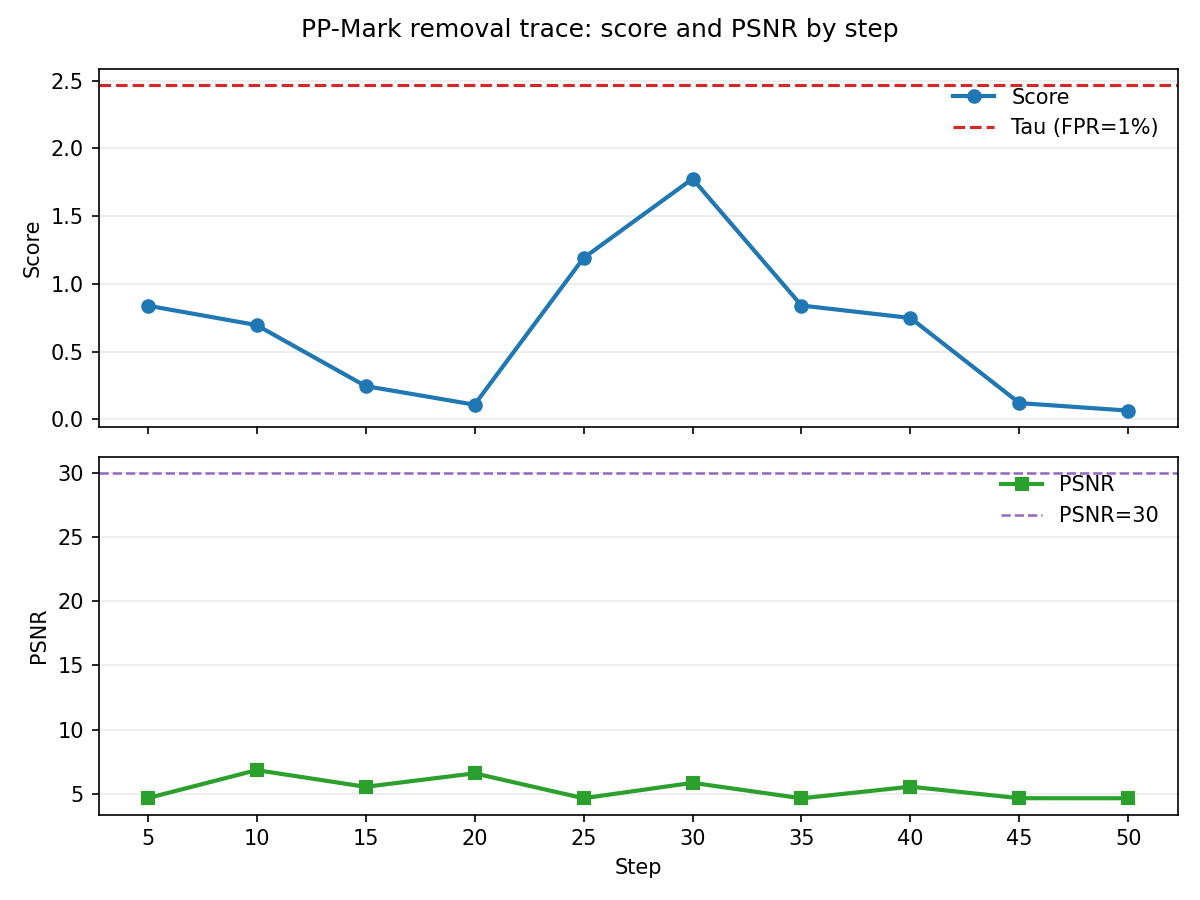
\includegraphics[width=0.82\textwidth]{figures/ch04_source_spsa_removal.png}
    \caption{SPSA removal trajectory}
    \label{fig:ch4-spsa-removal}
\end{figure}

In the complementary SPSA forgery test, score-mode FARs at 50, 100, and 150 steps
are 0.02, 0.00, and 0.01, with corresponding mean PSNRs 6.55, 6.61, and 6.63.
The aggregate FAR is 0.01 at mean PSNR 6.60.  The low-quality solutions again
show that reporting attack success without a perceptual constraint would be
misleading.  Full acceptance would additionally require a receipt for the changed
image.

\paragraph{Pixel and geometric transformations.}
The detector uses an alignment search for geometric synchronization.  Table
~\ref{tab:ch4-transformations} reports score-mode TPR for Stable Diffusion 2.1 and
SDXL.  Compression, blur, additive noise, and brightness changes retain TPRs from
0.86 to 1.00.  Random crop with resize is the weakest SDXL case at 0.74, while a
75-degree rotation reaches 0.85 on SD 2.1 and 0.97 on SDXL after synchronization.

\begin{table}[H]
    \centering
    \caption{Detection after pixel and geometric transformations}
    \label{tab:ch4-transformations}
    \small
    \setlength{\tabcolsep}{12pt}
    \renewcommand{\arraystretch}{1.15}
    \begin{tabular}{@{}lcc@{}}
        \toprule
        Transformation & SD 2.1 TPR & SDXL TPR \\
        \midrule
        JPEG, quality 25            & 0.94 & 1.00 \\
        Blur, \(8\times8\)          & 1.00 & 1.00 \\
        Gaussian noise, \(\sigma=0.1\) & 0.86 & 0.95 \\
        Brightness, \(\times0.6\)   & 0.98 & 1.00 \\
        Random crop and resize, 75\% & 0.87 & 0.74 \\
        Rotation, \(75^{\circ}\)    & 0.85 & 0.97 \\
        \bottomrule
    \end{tabular}

    \vspace{2pt}
    \parbox{0.92\textwidth}{\footnotesize
    Score-mode TPR at the matching 1\% FPR; SDXL crop-and-resize uses \(n=50\).}
\end{table}

These transformation results define the role of PP-Mark(score), not the validity
of an old proof.  The canonical SHA-256 image hash changes under every listed
operation.  A transformed image may still be discovered by the statistical
screen, but it becomes PP-Mark-accepted only after a producer issues a receipt for
that exact transformed pixel representation.

A post-submission sequential test applies 75\% crop, bicubic resize, and JPEG
quality 25 to the same 100 SD 2.1 watermarked images with no survivor filtering.
Persistent success requires detection at every checkpoint; 80 of 100 images remain
detectable through the complete pipeline, compared with 87 of 100 after crop--
resize alone and 94 of 100 after JPEG alone.  The 80\% result measures cumulative
score degradation under one fixed three-operation pipeline.  It does not change
the exact-image boundary of PP-Mark(accept).

\subsection{Efficiency, Image Quality, and Model Generalization}
\label{subsec:ch4-efficiency-generalization}

The sample count controls detector variance, proof work, and receipt size.  The two
source ablations appear in Figure~\ref{fig:ch4-sampling-tradeoff}.  Increasing the
count from 200 to 1000 reduces the empirical
score standard deviation from 0.1409 to 0.1301, a 7.7\% decrease; increasing it
from 1000 to 1500 supplies only a further 3.0\% decrease.  SP1 proving time grows
from 32.309 s at 200 samples to 48.572 s at 1000 and 60.272 s at 1500.  The
selected value of 1000 is therefore an empirical operating point rather than a
universal optimum.  Concentration with larger samples supplies the statistical
motivation, while the source analysis uses the registered empirical calibration
rather than claiming an asymptotic detector guarantee~\cite{hoeffding1963}.

\begin{figure}[H]
    \centering
    \begin{subfigure}[t]{0.48\textwidth}
        \centering
        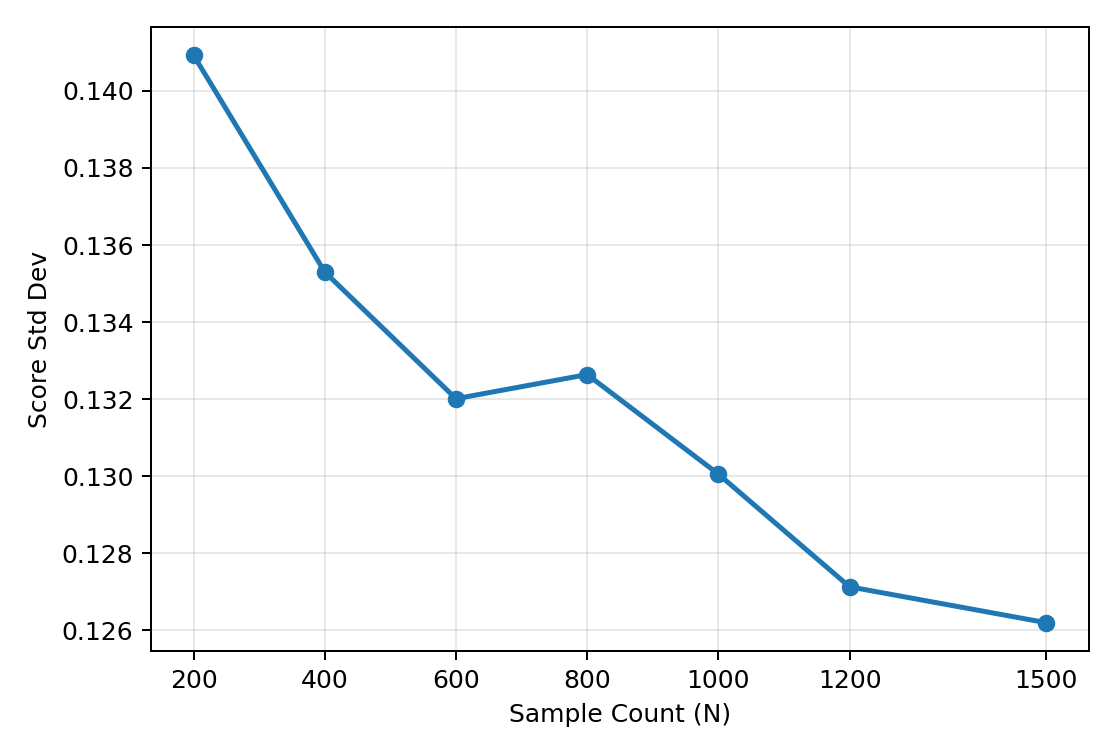
\includegraphics[width=\linewidth]{figures/ch04_source_sample_score_stability.png}
        \caption{Score variation}
        \label{fig:ch4-sample-score}
    \end{subfigure}
    \hfill
    \begin{subfigure}[t]{0.48\textwidth}
        \centering
        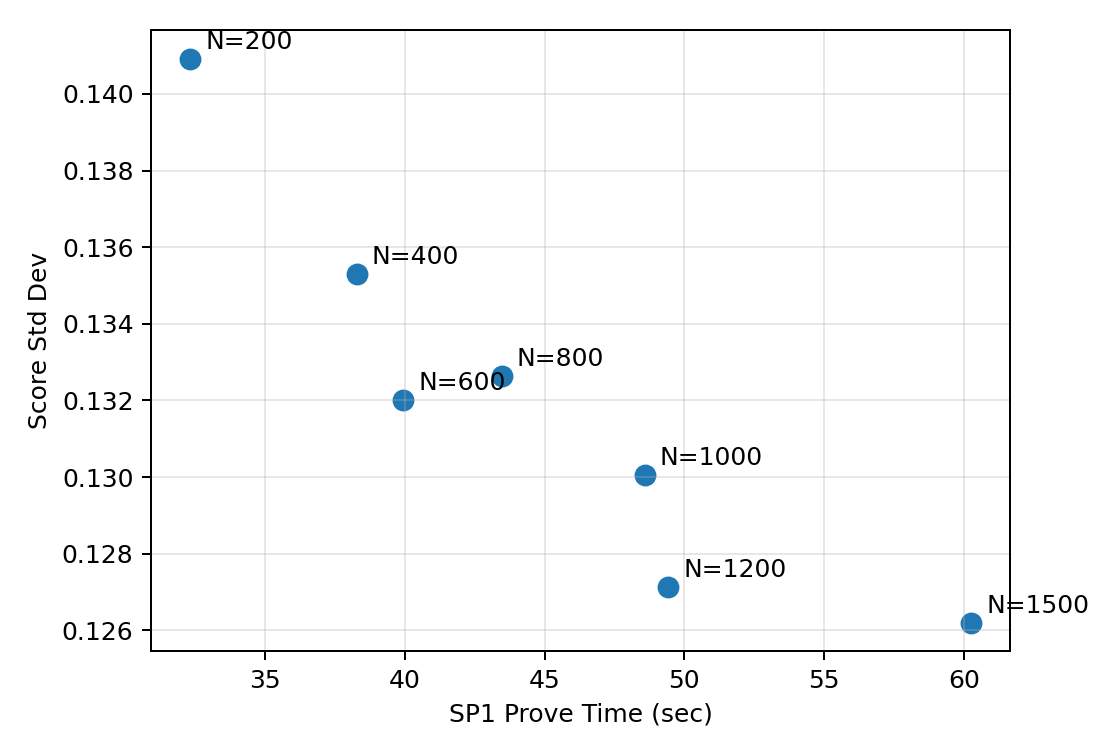
\includegraphics[width=\linewidth]{figures/ch04_source_score_proving_tradeoff.png}
        \caption{Proving time}
        \label{fig:ch4-score-proving}
    \end{subfigure}
    \caption{Sampling stability and SP1 proving trade-off}
    \label{fig:ch4-sampling-tradeoff}
\end{figure}

Table~\ref{tab:ch4-runtime} reports end-to-end runtimes on Stable Diffusion 2.1.
The score mode matches the Tree-Ring path at 0.89 s for embedding and 0.72 s for
verification.  Full acceptance adds 48.6 s for one-time proof generation and
7.59 s for receipt verification.  At
\(\PPSampleCount=1000\), the more precise SP1 checkpoints are 48.572 s proving
and 7.589 s verification, and the receipt occupies 40.68 MB.  The artifact is
therefore feasible for archival or on-request verification in the evaluated
environment, but it is costly for a per-upload streaming path.

\begin{table}[H]
    \centering
    \caption{End-to-end runtime on Stable Diffusion 2.1}
    \label{tab:ch4-runtime}
    \small
    \setlength{\tabcolsep}{15pt}
    \renewcommand{\arraystretch}{1.13}
    \begin{tabular}{@{}lcc@{}}
        \toprule
        Method & Embed or generate (s) & Verify (s) \\
        \midrule
        Tree-Ring        & 0.89 & 0.75 \\
        Gaussian Shading & 3.10 & 0.72 \\
        RingID           & 0.89 & 0.72 \\
        WIND             & 0.89 & 1.10 \\
        Stable Signature & 0.91 & 0.008 \\
        HiDDeN           & 0.001 & 0.001 \\
        TrustMark        & 0.013 & 0.004 \\
        InvisMark        & 0.002 & 0.009 \\
        PP-Mark(score)   & 0.89 & 0.72 \\
        PP-Mark(accept)  & \(0.89+48.6^{\dagger}\) & \(0.72+7.59^{\dagger}\) \\
        \bottomrule
    \end{tabular}

    \vspace{2pt}
    \parbox{0.92\textwidth}{\footnotesize
    \(^{\dagger}\)Additional SP1 proving and receipt-verification time at
    \(\PPSampleCount=1000\).}
\end{table}

After the submitted-paper evaluation, an SP1 v6.3.1 port with Merkle-work
optimization was rerun at the same \(\PPSampleCount=1000\) configuration.  It
reduced measured proving time from 48.572 s to 17.0 s and the receipt artifact from
40.68 MB to 2.81 MB.  This is reported as a post-submission implementation update,
not silently substituted into Table~\ref{tab:ch4-runtime} or the submitted attack
comparisons.  The update improves the engineering point but leaves the assurance
predicate and the distinction between routine score screening and one-time exact-
image proof generation unchanged.

Receipt size scales from 12.24 MB at 300 sampled positions to 65.96 MB at 1500;
the private witness grows from 254.69 KB to 1493.57 KB over the same range, while
the public input remains approximately 0.66 KB.  A STARK-to-SNARK wrapper or proof
aggregation could reduce distributed proof size, but that optimization is not
implemented or counted as a current result.

Embedding strength is selected with a tail-sensitive perceptual diagnostic.
Figure~\ref{fig:ch4-brisque} plots the 95th percentile of BRISQUE against
\(\alpha\).  Values from 3.0 through 4.0 remain approximately 34.1--34.9, whereas
4.5 rises to about 40.5.  The implemented \(\alpha=4.0\) retains the stronger
detection setting before this observed tail-quality degradation.  The underlying
study also reports KID 0.0011014 on one 500-image, 20-split configuration; because
that is one moderate-size setup, it is treated as supporting distributional
evidence rather than a definitive perceptual guarantee.

Post-submission matched-pool measurements place this result beside the evaluated
baselines in Table~\ref{tab:ch4-matched-quality}.  Lower BRISQUE is preferred,
KID is interpreted toward zero, and higher CLIP alignment is preferred.  PP-Mark
does not have the best value in every column; the defensible conclusion is that its
quality is comparable to several latent- and pixel-watermark baselines while its
full mode adds a different embedding-compliance guarantee.

\begin{table}[tbp]
    \centering
    \caption{Post-submission matched image-quality comparison}
    \label{tab:ch4-matched-quality}
    \footnotesize
    \setlength{\tabcolsep}{6pt}
    \renewcommand{\arraystretch}{1.10}
    \begin{tabular}{@{}lccc@{}}
        \toprule
        Method & BRISQUE p95 \(\downarrow\) &
        KID \(\times10^3\) \((\rightarrow0)\) & CLIP \(\times100\) \(\uparrow\) \\
        \midrule
        PP-Mark          & 34.14  & $1.101\pm0.202$   & 31.64 \\
        Gaussian Shading & 27.35  & $0.621\pm1.096$   & 32.42 \\
        HiDDeN           & 105.86 & $7.239\pm1.474$   & 31.30 \\
        InvisMark        & 31.36  & $-0.900\pm0.895$  & 32.53 \\
        RingID           & 34.64  & $-0.989\pm0.701$  & 32.41 \\
        Stable Signature & 32.69  & $-0.814\pm0.878$  & 32.50 \\
        Tree-Ring        & 41.90  & $-0.090\pm0.922$  & 32.30 \\
        WIND             & 27.42  & $-0.386\pm0.879$  & 32.28 \\
        TrustMark        & 29.44  & $-0.174\pm1.001$  & 32.54 \\
        \bottomrule
    \end{tabular}

    \vspace{2pt}
    \parbox{0.94\textwidth}{\footnotesize
    KID is an unbiased finite-sample estimator and can be slightly negative; such
    values are sampling estimates near zero, not negative distances.}
\end{table}

\begin{figure}[H]
    \centering
    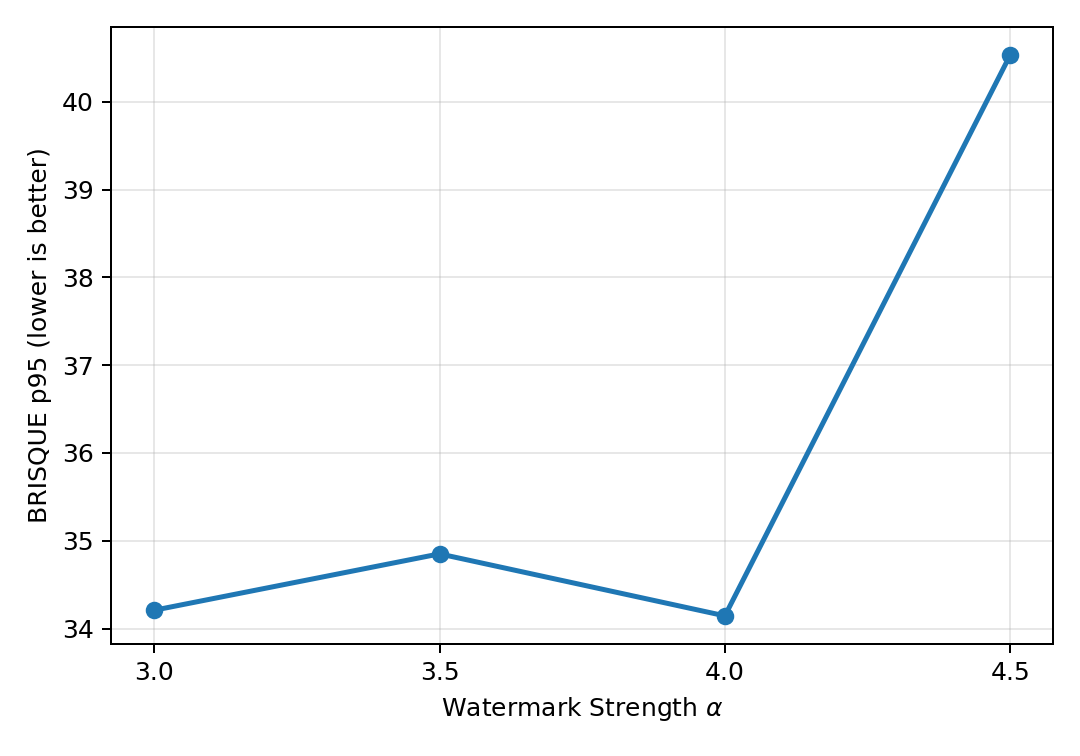
\includegraphics[width=0.78\textwidth]{figures/ch04_source_brisque_strength.png}
    \caption{Perceptual quality across embedding strengths}
    \label{fig:ch4-brisque}
\end{figure}

\paragraph{Inversion diagnostics.}
Assumption~\ref{ass:ch4-inversion-residual} is checked on 100 watermarked images
per latent-diffusion model.  On Stable Diffusion 2.1, the residual mean is
\(0.011\pm0.003\), the standard deviation is approximately 0.50, and the mean,
median, and maximum absolute residual--sign correlations are 0.30, 0.30, and
0.48.  The observed clean watermark score has mean 25.7 and minimum 17.4.  On
SDXL, the residual mean is \(-0.022\pm0.004\), with 95\% interval
\([-0.031,-0.013]\), standard deviation approximately 0.44, and mean, median, and
maximum absolute correlations 0.54, 0.55, and 0.66.  Correlation is stronger than
on SD 2.1, but it acts as shrinkage rather than complete cancellation in the
reported sample.

\paragraph{Bounded SDXL replication.}
The SDXL experiment uses 100 clean and 100 watermarked images per method, 50 DDIM
steps, \(\alpha=4.0\), and \(\PPSampleCount=1000\) on the 128-by-128 latent.
All thresholds are recalibrated to 1\% FPR on SDXL clean images.  PP-Mark's mean
watermarked score is 13.63 against \(\PPThreshold=2.47\), a 5.5-fold margin, and
all 100 clean watermarked evaluations cross the threshold.

Under Tree-Ring-sourced transfer, score-mode FARs at 50, 100, and 150 steps are
0.02, 0.00, and 0.01; under Gaussian-Shading-sourced transfer they are 0.01 at
every step.  The full mode records zero acceptances in all six conditions.  In the
SDXL white-box test, TrustMark and InvisMark each reach 1.00 FAR.  PP-Mark's score
mode reaches 0.11 with 95\% confidence interval 0.0562--0.1883, while the full
mode records 0.00.  These results show that the
registered construction can be run on two evaluated latent-diffusion models.
They do not establish architecture-agnostic generalization.

\paragraph{Limitations.}
Four limitations delimit the experimental conclusion.  First, proving time and
receipt size remain substantial at the selected sample count.  Second, the exact
image hash prevents unchanged receipt reuse after a benign edit; re-proving costs
about 48.6 s in the submitted environment and 17.0 s in the post-submission SP1
v6.3.1 update.  Third, the receipt must remain
attached or retrievable, and key rotation and revocation must operate correctly.
Fourth, geometric alignment remains imperfect for crop-and-resize on SDXL, and
only SD 2.1 and SDXL are tested.  The interface also does not account for
cumulative information exposed by repeated adaptive score queries.  That
dimension remains future work rather than a completed result in this chapter.

\section{Summary}
\label{sec:ch4-summary}

This chapter developed the \SecurePublicVerification{} axis of
\ClaimAlignedAssurance{}.  A hidden detector limits independent audit, whereas a
public detector exposes a score that can be queried or optimized.  PP-Mark
therefore keeps statistical screening separate from full acceptance, which
requires both image-side evidence and a publicly verifiable receipt.

The prompt hash, seed, model identifier, resolution, and producer-held key derive
a binding that determines the payload, sampled positions, Gaussian baselines, and
latent signs.  Q18 trace tuples are Merkle-committed, and the exact image hash
derives the post-commitment opening.  SP1 checks key binding, trace commitment,
the image-bound opening, and the opened embedding relation without disclosing the
secret key.

The two evidence layers remain experimentally distinct.  Search over 10,000
bindings defeats signature plus score, and white-box optimization raises the
public score on 76\% of the SD 2.1 covers, yet zero full acceptances are observed
in the reported forgery tests.  Score mode retains 0.74--1.00 TPR over the common
transformations and 0.98 after regeneration.  The exact-image proof is not
transform robust; an edited variant requires a new receipt.

The assurance statement remains conditional on hash resistance, SP1 soundness,
key control, the composite predicate, inversion behavior, and partial opening.
The circuit does not prove complete diffusion execution, semantic truth,
authorship, or legal identity.  Proof cost and persistence, key lifecycle,
geometric synchronization, two-model coverage, and adaptive queries remain
open limits.

Within those boundaries, PP-Mark demonstrates the chapter's central principle: a
public provenance claim should be released only when the visible detector outcome
and the registered verification evidence refer to the same context, signal,
image, and predicate.  Chapter~\ref{ch:conclusion} will combine this result with
the post-execution privacy audit to state the dissertation-wide principles of
Claim-Aligned Assurance.
